% method-comparision.tex
%
% Drafted by Juntang on August 22, 2024
%

\begin{frame}
  \frametitle{Comparison of Kernels}
        \begin{figure}
            \centering
            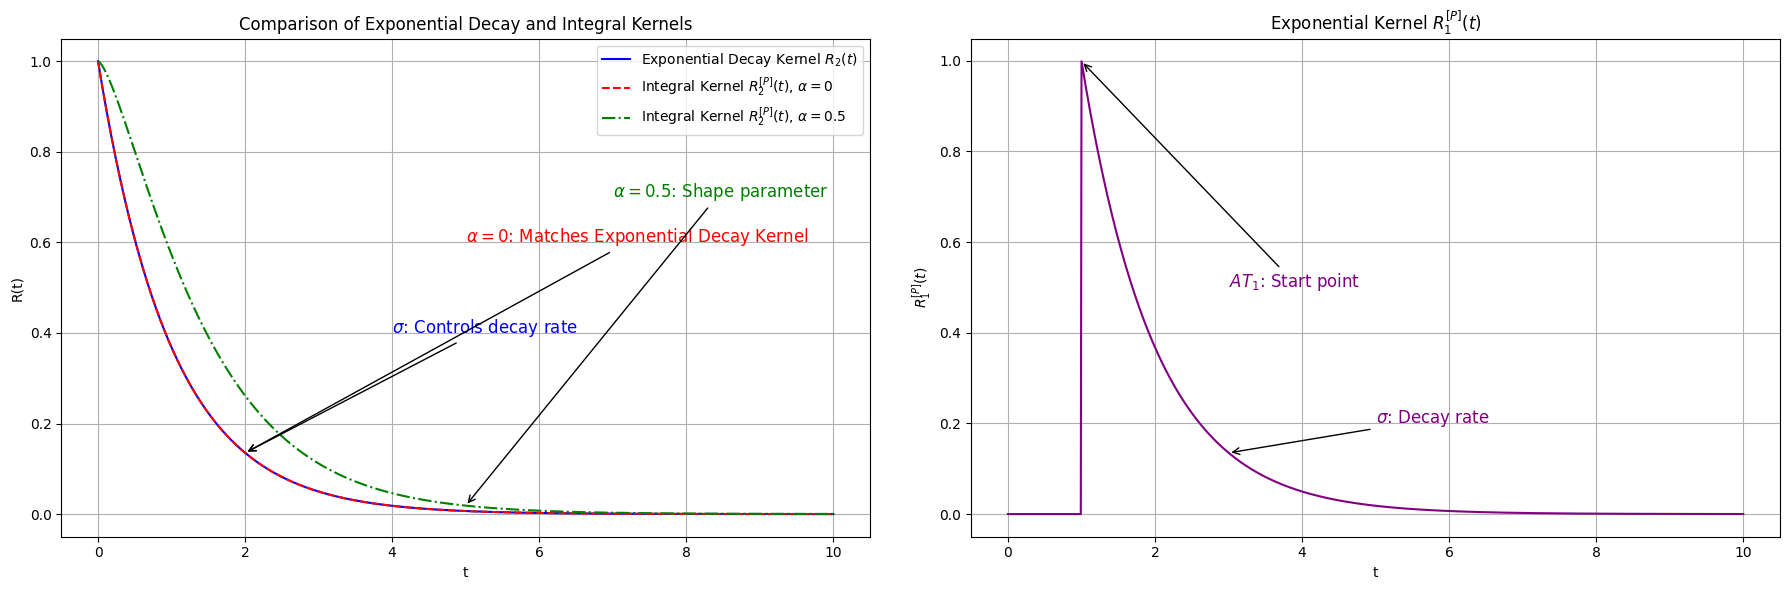
\includegraphics[width=\linewidth]{figures/method-compare.png}
            \caption{\textbf{Comparison of Kernel Functions.} 
            (Left) The plot compares the Exponential Decay Kernel \( R_2(t) \) (blue) with the Integral Kernel \( R_2^{[P]}(t) \) for two values of the shape parameter \(\alpha\): \(\alpha = 0\) (red, dashed), which matches the Exponential Decay Kernel, and \(\alpha = 0.5\) (green, dash-dotted), showing the effect of a non-zero \(\alpha\) on the kernel shape. The parameter \(\sigma\) controls the decay rate in both kernels. 
            (Right) The plot shows the Exponential Kernel \( R_1^{[P]}(t) \) (purple), which includes a shift controlled by \(AT_1\), illustrating how the start point and decay rate (\(\sigma\)) affect the kernel’s behavior.
            }
            \label{fig:comparision}
        \end{figure}
   

\end{frame}

%%% Local Variables:
%%% mode: latex
%%% TeX-master: "../topic-slide-main"
%%% End: